\documentclass[12pt]{article}
\usepackage{fancyhdr,listings,amsfonts,amsmath,color,lastpage}
\usepackage{float}
\usepackage{multirow}
\usepackage{enumitem}
\usepackage{caption}
\usepackage{tikz}
\usetikzlibrary{arrows.meta, positioning, shapes.geometric}

\tikzset{
    node style/.style={draw, rectangle, rounded corners, minimum width=3.5cm, minimum height=1.2cm, text centered, font=\sffamily},
    decision style/.style={draw, diamond, aspect=2, minimum width=3.5cm, text centered, font=\sffamily},
    arrow style/.style={->, thick},
}

% code listing settings
\usepackage{listings}
\lstset{
    language=Python,
    basicstyle=\ttfamily\small,
    aboveskip={1.0\baselineskip},
    belowskip={1.0\baselineskip},
    columns=fixed,
    extendedchars=true,
    breaklines=true,
    tabsize=4,
    prebreak=\raisebox{0ex}[0ex][0ex]{\ensuremath{\hookleftarrow}},
    frame=lines,
    showtabs=false,
    showspaces=false,
    showstringspaces=false,
    keywordstyle=\color[rgb]{0.627,0.126,0.941},
    commentstyle=\color[rgb]{0.133,0.545,0.133},
    stringstyle=\color[rgb]{01,0,0},
    numbers=left,
    numberstyle=\small,
    stepnumber=1,
    numbersep=10pt,
    captionpos=t,
    escapeinside={\%*}{*)}
}

\pagestyle{fancy}
\parindent0em

\newcommand{\masunitnumber}{CSC111}
\newcommand{\coursename}{Introduction to Computer Science}

% Header and footer
\lhead{}
\rhead{}
\chead{}
\lfoot{}
\rfoot{}
\cfoot{\thepage\ of \pageref{LastPage}}

\definecolor{listinggray}{gray}{0.9}
\lstset{backgroundcolor=\color{listinggray},rulecolor=\color{blue}}
\lstset{linewidth=\textwidth}
\lstset{commentstyle=\tt, stringstyle=\ttfamily,showspaces=false,basicstyle=\tt}
\lstset{showstringspaces=false, keepspaces=true}
\newcommand{\code}[1]{\lstinline@#1@}
\newcommand{\Code}[1]{\colorbox{listinggray}{\lstinline@#1@}}

\begin{document}

\setlength{\headsep}{14truemm}
\setlength{\headheight}{14truemm}
\setlength{\voffset}{-0.4truein}
\renewcommand{\headrulewidth}{0.0pt}

\begin{center}
    \textbf{UNIVERSITY OF ESWATINI} \\
    \textbf{DEPARTMENT OF COMPUTER SCIENCE} \\
    \vspace{0.5cm}
    \textbf{\masunitnumber\ -- \coursename} \\
    \textbf{RESIT EXAMINATION} \\
    \vspace{0.5cm}
    \textbf{SOLUTIONS MANUAL}
\end{center}

\vspace{1cm}
\noindent\textbf{Date:} 20 July 2026 \hfill \textbf{Time Allowed:} 3 Hours

\vspace{1cm}
\hrule
\vspace{0.5cm}

\section*{SECTION A: COMPULSORY (50 marks)}

\subsection*{Q1. Computer Science Disciplines} \hfill (10 marks)

\begin{enumerate}[label=(\alph*)]
    \item \textbf{Definition of Computer Science:} Computer Science is the study of computers and computational systems, focusing on software and software systems, including their theory, design, development, and application. It encompasses algorithm design, performance analysis, and solving complex computational problems beyond just programming. \hfill (2 marks)

    \textbf{Why more than programming:} It involves mathematical foundations, algorithm analysis, system design, human-computer interaction, and theoretical concepts such as computability and complexity, not merely writing code. \hfill (2 marks)

    \item \textbf{ACM Five Core Disciplines:} \hfill (6 marks -- 1 mark each for listing, 1 mark each for brief description)

    \begin{center}
    \begin{tabular}{|p{4cm}|p{9cm}|}
        \hline
        \textbf{Discipline} & \textbf{Brief Description} \\
        \hline
        Computer Engineering (CE) & Design and construction of computers and computer-based systems focusing on hardware, software, and communications. \\
        Computer Science (CS) & Wide range from theoretical foundations to cutting-edge developments; comprehensive foundation for adaptability. \\
        Information Systems (IS) & Integrating IT solutions with business processes to meet organizational needs effectively. \\
        Information Technology (IT) & Meeting user needs through selection, creation, and administration of computing technologies. \\
        Software Engineering (SE) & Developing reliable, efficient, and affordable software systems using engineering principles. \\
        \hline
    \end{tabular}
    \end{center}
\end{enumerate}

\bigskip

\subsection*{Q2. Computer Generations} \hfill (10 marks)

\begin{enumerate}[label=(\alph*)]
    \item \textbf{Third Generation (1964--1971):} \hfill (4 marks)
    \begin{itemize}
        \item \textbf{Technological breakthrough:} Integrated Circuits (ICs) -- transistors miniaturized on silicon chips.
        \item \textbf{Impact on accessibility:} Dramatically reduced size and cost, making computers accessible to mass audiences for the first time. Replaced punch cards and printouts with keyboards and monitors. First operating systems appeared, allowing multiple applications to run simultaneously.
    \end{itemize}

    \item \textbf{Any three generations (excluding 3rd):} \hfill (6 marks -- 2 marks each: 1 for technology, 1 for characteristic)

    \begin{itemize}
        \item \textbf{First Generation (1940--1956):} Technology -- Vacuum tubes; Characteristic -- Room-sized, extremely expensive, low reliability, used machine language.
        \item \textbf{Second Generation (1956--1963):} Technology -- Transistors; Characteristic -- Smaller, more reliable, introduced assembly and high-level languages (COBOL, FORTRAN).
        \item \textbf{Fourth Generation (1971--present):} Technology -- Microprocessors; Characteristic -- Desktop and portable computers, very affordable, high reliability, networks and internet.
        \item \textbf{Fifth Generation (present--beyond):} Technology -- Artificial Intelligence, quantum computing; Characteristic -- Natural language interfaces, parallel processing, still in development.
    \end{itemize}
\end{enumerate}

\bigskip

\subsection*{Q3. System Development Life Cycle (SDLC)} \hfill (10 marks)

\begin{enumerate}[label=(\alph*)]
    \item \textbf{Definition:} The SDLC is the formal process by which organizations build systems, providing a structured approach to system development from conception to maintenance. \hfill (2 marks)

    \item \textbf{Six phases:} \hfill (8 marks -- 1 mark for each phase name, 1 mark for each brief explanation)

    \begin{enumerate}
        \item \textbf{Preliminary Investigation (Feasibility Study):} Conduct preliminary analysis, propose alternative solutions, describe costs and benefits, submit preliminary plan with recommendations.
        \item \textbf{Systems Analysis:} Gather data, analyze the current system, determine what the system should do to meet user needs, write a report.
        \item \textbf{Systems Design:} Do preliminary design then detailed design, write a report with complete system specifications.
        \item \textbf{Systems Development:} Acquire software and hardware, test the complete system.
        \item \textbf{Systems Implementation:} Close coordination to make system workable and successful; training users; transitioning from old to new system.
        \item \textbf{System Maintenance:} Conduct audits, make periodic evaluations, make changes based on new conditions.
    \end{enumerate}
\end{enumerate}

\bigskip

\subsection*{Q4. Computer Literacy and Professionals} \hfill (10 marks)

\begin{enumerate}[label=(\alph*)]
    \item \textbf{Differentiate computer literacy vs computer competency:} \hfill (4 marks -- 2 marks each)

    \begin{itemize}
        \item \texttt{Computer literacy}: Having an understanding of what a computer is and how it can be used as a resource. Includes understanding computer fundamentals, knowledge of software types, awareness of different computer systems, and basic operational skills.
        \item \texttt{Computer competency}: Applying skills with computers to meet information needs and improve productivity. Includes transferring basic skills to new systems, adapting to different software environments, solving problems using computing tools, and enhancing personal and professional productivity.
    \end{itemize}

    \item \textbf{Differentiate computer professional vs computer user:} \hfill (6 marks -- 1 mark for each definition, 1 mark for each example)

    \begin{center}
    \begin{tabular}{|p{3.5cm}|p{5cm}|p{5cm}|}
        \hline
        \textbf{Aspect} & \textbf{Computer Professional} & \textbf{Computer User} \\
        \hline
        Definition & Knows technical aspects of using computers; designs and develops systems. & Person without extensive technical knowledge who uses computers for work or personal tasks. \\
        Examples & Software Engineer, System Analyst, Network Administrator, Database Administrator & Computer Operator, Data Entry Operator, Accountant, Administrative Clerk \\
        \hline
    \end{tabular}
    \end{center}
\end{enumerate}

\bigskip

\subsection*{Q5. Number Systems and Storage} \hfill (10 marks)

\begin{enumerate}[label=(\alph*)]
    \item $1101101_2$ to decimal: \hfill (3 marks)
    \[
    1\times2^6 + 1\times2^5 + 0\times2^4 + 1\times2^3 + 1\times2^2 + 0\times2^1 + 1\times2^0
    = 64 + 32 + 0 + 8 + 4 + 0 + 1 = \mathbf{109_{10}}
    \]

    \item $647_8$ to binary: \hfill (3 marks)
    $6 = 110$, $4 = 100$, $7 = 111$, so $\mathbf{110100111_2}$

    \item 3.5 GB to MB: \hfill (4 marks)
    \[
    1\text{ GB} = 1024\text{ MB}, \quad 3.5\text{ GB} = 3.5 \times 1024 = \mathbf{3584\text{ MB}}
    \]
\end{enumerate}

\newpage

\section*{SECTION B (50 marks)}

\subsection*{Q6. Algorithms and Flowcharts} \hfill (15 marks)

\begin{enumerate}[label=(\alph*)]
    \item \textbf{Definition and characteristics:} \hfill (5 marks -- 1 for definition, 1 each for any 5 characteristics)
    \begin{itemize}
        \item \textbf{Definition:} An algorithm is a step-by-step or sequential order of solving a problem or accomplishing a task.
        \item \textbf{Characteristics (any five):}
        \begin{enumerate}
            \item Must have a beginning and an end.
            \item Must be simple/clear for easy understanding.
            \item Must have an input.
            \item Must have a unique name.
            \item Must have an end result (desired output).
            \item Must be efficient and effective.
            \item Must be properly planned.
        \end{enumerate}
    \end{itemize}

    \item \textbf{Algorithm for cylinder volume and surface area:} \hfill (5 marks)
    \begin{verbatim}
    Step 1: Start
    Step 2: Input radius (r) and height (h)
    Step 3: Process:
        Step 3.1: Volume = 3.142 * r * r * h
        Step 3.2: TSA = (2 * 3.142 * r * r) + (2 * 3.142 * r * h)
    Step 4: Print Volume and TSA
    Step 5: Stop
    \end{verbatim}

    \item \textbf{Flowchart for admission:} \hfill (5 marks)
    \begin{center}
    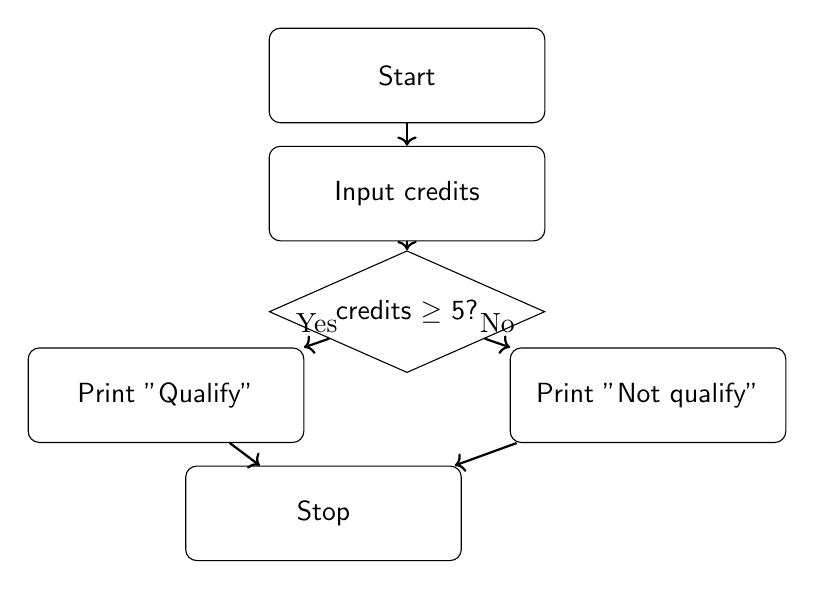
\begin{tikzpicture}[node distance=1.5cm, auto]
        \node (start) [node style] {Start};
        \node (input) [node style, below of=start] {Input credits};
        \node (decision) [decision style, below of=input] {credits $\ge$ 5?};
        \node (qualify) [node style, below left of=decision, xshift=-2cm] {Print "Qualify"};
        \node (notqual) [node style, below right of=decision, xshift=2cm] {Print "Not qualify"};
        \node (stop) [node style, below of=qualify, xshift=2cm] {Stop};

        \draw [arrow style] (start) -- (input);
        \draw [arrow style] (input) -- (decision);
        \draw [arrow style] (decision) -- node[above] {Yes} (qualify);
        \draw [arrow style] (decision) -- node[above] {No} (notqual);
        \draw [arrow style] (qualify) -- (stop);
        \draw [arrow style] (notqual) -- (stop);
    \end{tikzpicture}
    \end{center}
\end{enumerate}

\bigskip

\subsection*{Q7. Python Programming I} \hfill (15 marks)

\begin{enumerate}[label=(\alph*)]
    \item \textbf{Rectangle area and perimeter:} \hfill (7 marks)
    \begin{lstlisting}[numbers=none]
    # Program to calculate area and perimeter of a rectangle
    length = float(input("Enter length: "))
    width = float(input("Enter width: "))
    area = length * width
    perimeter = 2 * (length + width)
    print(f"Area: {area} square units")
    print(f"Perimeter: {perimeter} units")
    \end{lstlisting}
    \textit{Marking:} Input (2), calculations (2), formatted output with units (3).

    \item \textbf{String operations:} \hfill (8 marks)
    \begin{lstlisting}[numbers=none]
    s = input("Enter a sentence: ")
    print(s.upper())
    print(s.lower())
    print(len(s))
    print(s[:5])
    print(s[-5:])
    \end{lstlisting}
    \textit{Marking:} Input (1), each operation (1 each -- total 5), correct slicing (2 each for first and last, total 4) → total 8.
\end{enumerate}

\bigskip

\subsection*{Q8. Systems Analysis and Design} \hfill (20 marks)

\begin{enumerate}[label=(\alph*)]
    \item \textbf{System definition and six elements:} \hfill (6 marks -- 1 for definition, 1 each for elements)
    \begin{itemize}
        \item \textbf{Definition:} A collection of related subsystems/components that interact to perform a task to accomplish a goal.
        \item \textbf{Elements:} Outputs, Inputs, Processor(s), Control, Feedback, Environment and Boundaries.
    \end{itemize}

    \item \textbf{Five reasons for system failure:} \hfill (5 marks -- 1 each)
    \begin{enumerate}
        \item Lack of communication among users, management, and specialists.
        \item Politics and hidden motives.
        \item Lack of management support.
        \item Technological incompetence.
        \item Lack of user training.
    \end{enumerate}

    \item \textbf{Importance of documentation:} \hfill (5 marks -- any 4 reasons, 1 each)
    \begin{itemize}
        \item Aid analysis – facilitates system understanding and problem diagnosis.
        \item Aid design – provides design reference and guides development.
        \item Aid communication – ensures consistent understanding among team members.
        \item Aid training – provides training material for new users.
        \item Future developments – supports system evolution and upgrades.
        \item Maintenance – enables effective troubleshooting and system upkeep.
        \item User consumption – provides user manuals and operating procedures.
    \end{itemize}

    \item \textbf{System software vs Application software:} \hfill (4 marks -- 2 marks each for definition, 1 mark each for examples)

    \begin{center}
    \begin{tabular}{|p{4cm}|p{5.5cm}|p{5.5cm}|}
        \hline
        \textbf{Aspect} & \textbf{System Software} & \textbf{Application Software} \\
        \hline
        Definition & Manages computer resources and provides basic functionality. & Performs tasks that directly benefit the user. \\
        Examples & Operating Systems (Windows, Linux), utility programs, device drivers & Word processors, spreadsheets, database systems, games \\
        \hline
    \end{tabular}
    \end{center}
\end{enumerate}

\newpage

\section*{SECTION C (50 marks)}

\subsection*{Q9. 8-bit Binary Arithmetic} \hfill (15 marks)

Given: $A=25_{10}$, $B=2F_{16}$, $C=43_8$, $D=-14_{10}$.

\begin{enumerate}[label=(\alph*)]
    \item $D = -14_{10}$ in 2's complement: \hfill (3 marks)
    \begin{enumerate}
        \item $14_{10} = 00001110_2$ (8-bit)
        \item 1's complement: $11110001_2$
        \item 2's complement: $11110001 + 1 = \mathbf{11110010_2}$
    \end{enumerate}

    \item \textbf{Binary sum of A and B:} \hfill (4 marks)
    $A = 25_{10} = 00011001_2$ \\
    $B = 2F_{16} = 00101111_2$ (since $2F_{16} = 47_{10}$) \\
    Sum: $00011001 + 00101111 = 01001000_2$ (no overflow). \\
    $\mathbf{01001000_2}$

    \item $A - B$ using 2's complement: \hfill (4 marks)
    $A = 00011001_2$ \\
    $B = 00101111_2$; 2's complement of B = $11010001_2$ \\
    $A + (-B) = 00011001 + 11010001 = 11101010_2$ \\
    Result: $\mathbf{11101010_2}$ (which is $-22_{10}$, correct).

    \item \textbf{Can $-150_{10}$ be represented?} \hfill (4 marks)
    Range of 8-bit 2's complement: $-128$ to $+127$. \\
    Since $-150 < -128$, it \textbf{cannot be represented}. \\
    Justification: with 1 sign bit and 7 magnitude bits, the maximum magnitude is 127.
\end{enumerate}

\bigskip

\subsection*{Q10. Python Programming II} \hfill (15 marks)

\begin{enumerate}[label=(\alph*)]
    \item \textbf{Temperature converter:} \hfill (8 marks)
    \begin{lstlisting}[numbers=none]
    temp = float(input("Enter temperature: "))
    choice = input("Convert from C or F? ")
    if choice.upper() == 'C':
        f = (temp * 9/5) + 32
        print(f"{temp}°C = {f:.2f}°F")
    elif choice.upper() == 'F':
        c = (temp - 32) * 5/9
        print(f"{temp}°F = {c:.2f}°C")
    else:
        print("Invalid choice")
    \end{lstlisting}
    \textit{Marking:} Input (2), if/elif structure (2), correct formulas (2), formatted output (2).

    \item \textbf{Multiplication table:} \hfill (7 marks)
    \begin{lstlisting}[numbers=none]
    num = int(input("Enter a number: "))
    for i in range(1, 11):
        print(f"{num} × {i} = {num * i}")
    \end{lstlisting}
    \textit{Marking:} Input (1), loop (2), calculation (2), formatting (2).
\end{enumerate}

\bigskip

\subsection*{Q11. Computer Architecture and Number Systems} \hfill (20 marks)

\begin{enumerate}[label=(\alph*)]
    \item \textbf{Stored program concept:} \hfill (5 marks)
    The concept (proposed by John Von Neumann, 1944--45) states that programs and data are logically the same and are stored in the same memory. This allows programs to be loaded and executed automatically, enabling reprogrammability and flexibility. It is the foundation of modern computer architecture.

    \item \textbf{RAM vs ROM:} \hfill (5 marks)

    \begin{center}
    \begin{tabular}{|p{3.5cm}|p{5cm}|p{5cm}|}
        \hline
        \textbf{Aspect} & \textbf{RAM} & \textbf{ROM} \\
        \hline
        Volatility & Volatile (data lost on power off) & Non-volatile (retained) \\
        Usage & Temporary working space for programs and data & Permanent instructions (e.g., BIOS) \\
        Read/Write & Read and Write & Read only (mostly) \\
        \hline
    \end{tabular}
    \end{center}

    \item \textbf{Role of Control Unit (CU):} \hfill (5 marks)
    The Control Unit coordinates all program instructions, directs signal movement, manages communication between memory, I/O and ALU, controls operation speed and timing, decodes instructions, and acts as the ``traffic controller'' of the CPU.

    \item \textbf{Conversions:} \hfill (5 marks)
    \begin{enumerate}
        \item $3A7_{16}$ to binary: $3 = 0011$, $A = 1010$, $7 = 0111$ $\Rightarrow \mathbf{001110100111_2}$ (or $1110100111_2$). \hfill (3 marks)
        \item $158_{10}$ to octal: $158 \div 8 = 19$ remainder 6, $19 \div 8 = 2$ remainder 3, $2 \div 8 = 0$ remainder 2 $\Rightarrow \mathbf{236_8}$. \hfill (2 marks)
    \end{enumerate}
\end{enumerate}

\vspace{1cm}
\begin{center}
    \textbf{END OF SOLUTIONS MANUAL}
\end{center}

\end{document}